\newtheorem*{drs}{Descartes' rule of signs (DRS)}
\newtheorem*{gp}{Gauss' property}
\newtheorem*{tiv}{Theorem of the intermediate values (TIV)}

\subsection{Descartes' rule of signs}

In his 1637 treaty called "La Géométrie", 
René Descartes expressed a rule allowing to estimate 
the number $c$ of positive real roots of a univariate 
polynomial, which we commonly call the Descartes's rule of signs. 
Later, in 1828, Carl Friedrich Gauss proved that if we count 
the roots with their multiplicities, then the number of positive roots 
has the same parity as $c$. 
Usually, Descartes' rule of signs  refers also to the enhancement of Gauss.

\begin{drs}
Let us consider a univariate polynomial $P\in\mathbb{R}[X]$ and the sequence 
$(a_n)$ of its non-zero coefficients. Let $c$ be the number of sign changes 
of the sequence $(a_n)$. Then the number of positive roots of $P$ is at most $c$.
\end{drs}


\begin{gp}
If we consider the previous rule of signs and 
count the roots with their multiplicities, 
then the number of positive real roots of $P$ 
has the same parity than $c$.
\end{gp}

\noindent \textit{Consequence:} We can also find the number of 
negative real roots applying Descartes' rule of signs to $Q(X) = P(-X)$.


This easy rule is the pillar of the reasoning in our work. 
Indeed, deciding where the real roots of a polynomial are located
reduces to the problem  of counting the number of real roots
of a polynomial in an interval.
The example of Section 2.3 illustrates this process.
The following basic theorem plays an essential role in the proof
of Descartes' rule of signs.


\begin{tiv}
If $f$ is a real-valued continuous function on the interval $[a, b]$ and $u$ is a number between $f(a)$ and $f(b)$, then there exists $c\in [a, b]$ such tha we have $f(c) = u$.
\end{tiv}


In particular if $u = 0$, then there  exists $c\in [a, b]$ such that $f(c) = 0$ holds.


\subsection{Horner's method}

This well-known high school tricks is used for evaluating a polynomial
efficiently.
Instead of considering $P(X) = \sum_{i=0}^{n} a_i\, X^i = a_0 + a_1\, X + a_2\, X^2 + ... + a_n\, X^n$, we write $P$ as
$$P(X) = a_0 + X\, \left(a_1 + X\, \left(a_2 + X\,\left(\cdots \left(a_{n-1} + \left(a_n\, X\right)\cdots \right)\right)\right)\right).$$
This allows one to reduce the number of coefficient operation
necessary to evaluate $P(X)$ at a point 
from ${\Theta}(n^2)$ to  ${\Theta}(n)$.\\
 


\textit{\textbf{Example :}}
Let us consider $P(X) = 3\, X^3 - 5\,X^2 - 3\,X + 2$. We want to calculate $P(4)$ by hand.\\
\underline{Naive method :} $P(4) = 3\times 4^3 - 5\times 4^2 - 3\times 4 + 2$\\
So $P(4) = 3\times 4^3 - 5\times 16 - 12 + 2 = 3\times 16\times 4 - 80 - 10 = 3\times 64 - 90 = 192 - 90 = 102$\\
\underline{Horner's method :} $P(X) = 2 + X\, \left(-3 + X\, \left(-5 + 3\,X \right) \right)$\\
So :
$ P(4) = 2 + 4\, \left(-3 + 4\, \left(-5 + 3\,4 \right) \right) = 2 + 4\, \left(-3 + 4\times 7 \right) = 2 + 4\times 25 = 102 $\\

\subsection{Example}
Let us consider $P(X) = X^3 + 3\, X^2 - X - 2$.\\
According to the Descartes' rule of signs, $c = 1$ so $P$ has $1$ positive root.\\
Let us consider $Q(X) = P(-X) = -X^3 + 3\, X^2 + X - 2$, here $c = 2$ so $P$ has either $2$ either $0$ negative roots. We have $P(-1) = 1$ and $\lim_{X \to -\infty} P(X) = -\infty$ so there exists $r_{1}\in ]-\infty; -1[\, |\, P(r_1) = 0$, then we deduce that there are exactly $2$ negative roots.\\
Using the TIV for $u = 0$, we can refine these intervals, calculating $P$ at some real numbers : \\
As $P(-1) = 1$ and $P(-2) = -2$, then $r_1\in ]-2, -1[$.\\
As $P(0) = -2$ and $P(-1) = 1$, then the second negative root $r_2\in ]-1;0[$.\\
As $P(0) = -2$ and $P(1) = 1$, then the positive root is $r_3\in ]0, 1[$.


\subsection{Vincent Collins Akritas Algorithm}
To isolate the real roots of a polynomial $P$, our objective is to use the Vincent-Collins-Akritas (VCA) Algorithm which computes a list of disjoint intervals with rational endpoints such that each real root of $P$ belongs to a single interval and each interval contains only one real root of $P$. As mentioned above, the problem of isolating the real roots of $P$ and that of counting its real roots are essentially the same. Therefore, if an algorithm solves one of these two problems, then is solves the other. The following Algorithm 1  (taken from~\cite{CacheComp}) uses Algorithm 2 and shows how we can reduce the search  for the roots in $\mathbb{R}$ to the search of the roots in $\left]0, 1\right[$.

\begin{center}
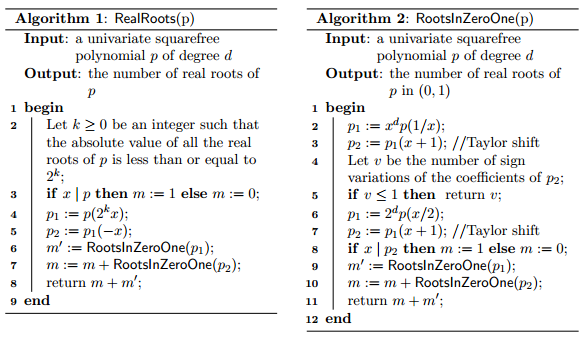
\includegraphics[scale=1]{VCAalgo.png}
\end{center}

Algorithm 1 calls several times the procedure RootsInZeroOne 
which, itself,  performs several times a Taylor shift by 1
(usually called Taylor shift). 
The Taylor shift by $a\in\mathbb{R}$ of a polynomial $P$ 
consists of computing the coefficients of the
polynomial $P(x+a)$ in the monomial basis.
 We will see later what there are differents ways to do this Taylor shift by 1.
Even if evaluating $P(x+1)$ seems an operation mathematically trivial,
non-triavial algorithms have been developed to perform
this operation efficiently on polynomials of large degrees.\\

Since the dominant computational costs of the VCA Algorithm
comes from the Taylor shift by 1, it is natural
to optimize this operation, in particular, in terms
of parallelism and data locality.
Of ourse Algorithms 1 and 2, with their divide and conquer 
scheme, seem to provide additional opportunities
for concurrent execution.
However, the work load in the recursive calls of Algorithms 1 and 2
is generally largely unbalanced, thus, leading to very little
parallelism in practice.
